%% by Michael Shell
%% Edited by Dominic Carr
%%
%% This work is distributed under the LaTeX Project Public License (LPPL)
%% ( http://www.latex-project.org/ ) version 1.3, and may be freely used,
%% distributed and modified. A copy of the LPPL, version 1.3, is included
%% in the base LaTeX documentation of all distributions of LaTeX released
%% 2003/12/01 or later.
%% Retain all contribution notices and credits.

\documentclass[10pt,journal,compsoc]{IEEEtran}

\hyphenation{op-tical net-works semi-conduc-tor}

\usepackage{lipsum} 
\usepackage{hyperref}
\usepackage{biblatex}
\usepackage{graphicx}
\usepackage{listings}
\usepackage{xcolor}




\graphicspath{{images/}}

\addbibresource{test.bib}


\begin{document}
% paper title
% Titles are generally capitalized except for words such as a, an, and, as,
% at, but, by, for, in, nor, of, on, or, the, to and up, which are usually
% not capitalized unless they are the first or last word of the title.
% Linebreaks \\ can be used within to get better formatting as desired.
% Do not put math or special symbols in the title.
\title{ Evaluating React.js Against Competing Frameworks}

% author name
\author{David Amankwah% <-this % stops a space
}

% The paper headers
\markboth{Research Methods in Computing \& IT - Literature Review}%
{}

\IEEEtitleabstractindextext{
    \begin{abstract}
        This literature review examines the capabilities of React, Angular and Vue in the realm of web application development. The research papers explore the concepts and the features of React, Angular, Vue to determine the best framework for developers to build responsive web applications. React is an emerging and widely used framework among developers because it offers many features for front-end development. A comparative analysis with Angular and Vue shows the capabilities of React. The different aspects of React are compared to Angular and Vue to decide whether it is the best solution for web development. 
    \end{abstract}
}

% make the title area
\maketitle

\label{sec:introduction}
\section{Introduction}
\IEEEPARstart{T}{he} purpose of a web application is to provide the best user experience, continuing to replace legacy desktops \cite{kaluvza2018comparison}. An attractive, responsive web application is required and stands at the forefront of this evolution \cite{kaluvza2018comparison}. Building an effective project requires a framework to streamline important
aspects. \textbf{The best way to develop} a project are using frameworks to simplify many aspects for us, such as code structure and maintenance \cite{vyas2022comparative}. A framework is crucial for developers to handle difficult task easily.


\subsection{Role of Front-End Libraries/Frameworks, and React.js}
According to Carl Lawrence Mariano from the Dublin Institute of Technology \cite{mariano2017benchmarking}, JavaScript is a well known programming language used for advanced web design. JavaScript frameworks and libraries allow you to design unique, responsive, and creative web applications with front-end implementations of HTML and CSS style\cite{mariano2017benchmarking}. Frameworks and libraries help developers better manage their coding and ease the complexity of developing these applications \cite{mariano2017benchmarking}. React is a prominent JavaScript front-end library designed by Facebook. It provides a declarative, high performance and maintainability \cite{chen2019front}. This approach is beneficial for developers when creating a user interfaces. React employs a Virtual DOM and displays changes when the state is updated \cite{chen2019front}. React will make sure rendering and logic are present in the component, without any interfering with other functions \cite{chen2019front}. Improved usability and performance make the React library a strong versatile option for developing modern web applications \cite{chen2019front}.


\subsection{ Purpose of the Literature Review}
Web applications are an ever-evolving field. The purpose of this literature review is to explore and understand React, the well-known JavaScript front-end library, comparing its tools and features to other web application technologies. Through analysis and discussion, the reviews aim to provide insightful information on how React compares to other web applications.

\section{Introduction to React.js}
React is a popular JavaScript front-end library because it lets developers to build responsive and attractive web applications, with a range of tools. React abstracts the Document Object Model (DOM), which offers a simple, performing and robust application development experience \cite{aggarwal2018modern}. The core concepts of using React are Virtual DOM, JSX and components.


\subsection{The core concepts of React}

The virtual DOM is one of the most useful features of React. The virtual act as a lightweight representation of the DOM. The virtual DOM allows React.js developers to handle JavaScript as reactive \cite{dinku2022react}. The virtual DOM is able to  re-render every state change, reflecting user activities and providing a fluid user experience \cite{dinku2022react}. Virtual DOM is a groundbreaking feature for updating specific components. The basic part of using React is components. Components are independent, reusable and encapsulated visual elements with specific functions. There are two types of components, namely class components and functional components \cite{lazuardy2022modern}. Class components support state management and contain a life cycle, with separate callback APIs for each life cycle event \cite{dinku2022react}. JSX stands for JavaScript XML and extends JavaScript to develop React.js components as simple as building HTML pages \cite{dinku2022react}. It adds HTML structures using JavaScript code. React uses components, JavaScript XML, and virtual DOM to create a powerful user interface. These features are integrated to support the development process for front-end developers.
\begin{figure}[ht]
    \centering
    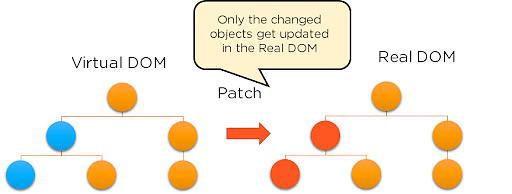
\includegraphics[width=0.45\textwidth]{V-RDOM.jpg}
    \caption{DOM tree updated \cite{vyas2022comparative}}
    \label{fig:dom}
\end{figure}React maintains two virtual DOMs, one of which is an updated and the other is simply the pre-updated version of the updated version \cite{vyas2022comparative}. The batch updates used by React allow the batch of changes to transfer the actual DOM instead of updating a component state's changes one by one \cite{vyas2022comparative}. React ensure that to the actual DOM picks up the batch changes to re-render the user interface design, which makes it very effective at managing an expensive component process \cite{vyas2022comparative}. React will create operations that execute on the real DOM with less stress, which is why for React is very quick. \cite{wohlgethan2018supportingweb}.


\section{Overview of Responsive Web Application Technologies}
Angular and Vue are two JavaScript frameworks that play a vital role in dynamic web application development. They have different properties and features. Angular and Vue offer functioning solutions to creating a quality web designs. Front end developers have these options to build stand out web applications.

\subsection{Vue Framework}
Vue is known to be a progressive framework. Vue is capable of building a user interface. It is suitable for both small projects and large scale single page
application\cite{wohlgethan2018supportingweb}. It can also provide an implementation of plugins and custom behaviours. Vue is a evolving and expanding framework with many capabilities for front end developers\cite{filipova2016learning}.Vue offers a range of features to have a hand in developing a modern web application. Vue offers developers a reactivity model to design user interfaces. According to Aylar Meredova \cite{meredova2023comparison}, Vue data is stored in a reactive data object, which is watched by a reactive system. When a changes are made to the data object, Vue automatically updates the user interface to reflect the new data\cite{meredova2023comparison}. A reactivity model is a core feature of Vue for designing a responsive user interface. Vue allows you to create custom directives with a mechanism to enable custom behaviour of DOM to data mapping \cite{filipova2016learning}. This feature is useful for flexibility and customization. Vue have methods to manipulate data, and take logic and store it in a reusable way so that it can use it multiple times without repeating the code \cite{macrae2018vue}. Vue also allows developers to pass options object to an instances, and all the properties found in that object are added to the Vue’s reactivity system \cite{cincovic2020comparison}.

\subsection{Angular Framework}
Angular is a front-end framework developed by Google that can be used to create functional single-page applications. Angular empowers traditional HTML by extending its current vocabulary, to develop expressive, reusable, and maintainable application components\cite{branas2014angularjs}. Angular has routing that provides a dynamic routing system for developers. This can help create navigation in the web application. Routes depend on the ngRoute module and the application requires it to be started \cite{williamson2015learning}. Dependency Injection is a feature built into Angular libraries for component and service management. Dependency Injection makes an application more testable, as it is one main advantage of using AngularJS \cite{williamson2015learning}. Directives in Angular allow you to add some behavior to HTML elements. Angular comes with many directives that helps you define the view for your app, and how your application works to create reusable components \cite{green2013angularjs}. These features highlight the strengths and versatility of Angular. 


\section{Comparison with Other Technologies}
React has become one of the most prominent responsive web technologies. It offers many unique and dynamic features to help you learn to code. Angular and Vue have also become strong web technologies for front-end development. The objective of this analysis is to determine which web technology offers the most in terms of learning, performance, flexibility and community support. 

\subsection{Ease of Learning}
React is popular because it is very simple to use. However, React requires developers to know JavaScript. React uses
JSX and this can be challenging to the developers \cite{cincovic2020comparison}. This can be difficult for developers starting out with React and creating a new project. Angular also has a steep learning curve with Typescript, and Vue has the smallest learning curve because it doesn't require
anything else but basic front-end technologies such as HTML, CSS and JavaScript \cite{cincovic2020comparison}. Angular takes time to learn the features it provides, and can be very limiting for some developers because it makes options up front for developers about how to handle certain situations  \cite{wohlgethan2018supportingweb}. React need developers to have in-depth knowledge of JavaScript because developers need to be able to modify JSX code in order to change structural
or styling related parts \cite{wohlgethan2018supportingweb}. Vue mainly uses ES6 for simple code development, and uses only the core web technologies, so no additional compiler is required \cite{wohlgethan2018supportingweb}. Beginner developers can expect to find Vue easier to learn than React and Angular on the first try. Let's examine these technologies based on key factors to offer a comprehensive comparison. 

\begin{table}[ht]
    \centering
    \begin{tabular}{llr}
        \hline
        \multicolumn{2}{c}{\textbf{Factor}} \\
        \cline{1-2}
        \textbf{Ease of Learning} & \\
        React.js & Average \cite{cincovic2020comparison}\\
        Angular & Steeper learning curve \cite{wohlgethan2018supportingweb}\\
        Vue.js & Small learning curve\cite{wohlgethan2018supportingweb} \\
        \hline
    \end{tabular}
    \caption{Comparison of React.js, Angular, and Vue.js}
    \label{tab:comparison}
\end{table}

\subsection{Performance}
When developing small web applications, Vue is more suitable to work with because it is smaller than React and Angular. However, Angular, React and Vue all offer equally-sized code bundles with effective techniques such as lazy loading supported by all three  \cite{vyas2022comparative}. Both React and Vue employ a virtual DOM to update changes in the real DOM, making them very fast and efficient. Angular uses the real DOM and is therefore slower than React and Vue \cite{vyas2022comparative}. Directives in Angular allow you to define the root of elements, manipulating the elements to make the coding process robust \cite{branas2014angularjs}. Vue directives allow developers to use templates to display data on the page \cite{macrae2018vue}. This is an approach that helps prevent code from being responsible for deciding whether to show or hide the elements in JavaScript \cite{macrae2018vue}. React combines user interface design and JavaScript logic to create the JSX, which is a concept that Angular and Vue have never done before \cite{vyas2022comparative}. The table below examines the technologies based on the key factors provided.

\begin{table}[ht]
    \centering
    \begin{tabular}{llr}
        \hline
        \multicolumn{2}{c}{\textbf{Factor}} \\
        \cline{1-2}
        \textbf{Performance} & \\
        React.js & Efficient virtual DOM \cite{vyas2022comparative}\\
        Angular & Robust coding \cite{branas2014angularjs}\\
        Vue.js & Good for smaller project\cite{vyas2022comparative}\\
        \hline
    \end{tabular}
    \caption{Comparison of React.js, Angular, and Vue.js}
    \label{tab:comparison}
\end{table}

\subsection{Flexibility}
When it comes to flexibility, Angular is very strict, React and Vue are much more flexible when building a web application \cite{cincovic2020comparison}. Angular provides everything included in the package and the defined code architecture is limited \cite{cincovic2020comparison}. However, React and Vue are have no limitations in application structure and combine well with other libraries \cite{cincovic2020comparison}. React allows developers to use Redux, a state management library that combines Flux, Command pattern and Elm design \cite{chen2019front}. Vue allows developers to configure HTML dynamically by using an automatic built-in HTML escaping, allowing the text in your HTML to be displayed without escaping \cite{macrae2018vue}. Vue would use a single file components, but like Angular, it separates templates and JavaScript logic apart \cite{vyas2022comparative}. The table below examines the key factors.

\begin{table}[ht]
    \centering
    \begin{tabular}{llr}
        \hline
        \multicolumn{2}{c}{\textbf{Factor}} \\
        \cline{1-2}
        \textbf{Flexibility} & \\
        React.js & Flexible \cite{cincovic2020comparison}\\
        Angular & Not flexible \cite{cincovic2020comparison}\\
        Vue.js & Flexible \cite{cincovic2020comparison}\\
        \hline
    \end{tabular}
    \caption{Comparison of React.js, Angular, and Vue.js}
    \label{tab:comparison}
\end{table}

\subsection{Community Support}
React has the advantage of having the largest community support, Angular is in second place and Vue is in third place \cite{cincovic2020comparison}. React and Angular were expected to receive the most support from the community since they were developed by two large companies such as Google and Facebook, and Vue was developed by a small team led by Evan You \cite{cincovic2020comparison}. Developers usually faces many problems when using Angular compared to React and Vue \cite{wohlgethan2018supportingweb}. Stack Overflow is an online tool that helps developer to find solutions related to Angular, React and Vue \cite{dinku2022react}. Developers appreciates React, but Angular is the most dreaded framework by developers \cite{wohlgethan2018supportingweb}. The table below examines the key factors.

\begin{table}[ht]
    \centering
    \begin{tabular}{llr}
        \hline
        \multicolumn{2}{c}{\textbf{Factor}} \\
        \cline{1-2}
        \textbf{Community Support} & \\
        React.js & Largest, More than Angular \cite{cincovic2020comparison}\\
        Angular & Large, More than Vue  \cite{cincovic2020comparison}\\
        Vue.js & Smaller \cite{cincovic2020comparison}\\
        \hline
    \end{tabular}
    \caption{Comparison of React.js, Angular, and Vue.js}
    \label{tab:comparison}
\end{table}

\subsection{Comparison overview}
In summary, each technology has its strengths and weaknesses for creating robust web applications. React and Vue have the upper hand in some cases, but Angular has its advantages for front-end developers. Developers must ensure that the project specific requirements and structure are appropriate for the chosen web technology.

\section{Cases and Examples}
React is a very versatile and powerful library for building user interfaces. There are situations where React is used to code responsive web applications. React and Vue mainly use JavaScript, while Angular uses Typescript. The following comparison explores the three different web technologies codes to see how they benefits for developers.

\subsection{React cases}
Compared to Angular, where a component's the logic and template for are in separate files, React keeps the two closely related and its components has both logic and templates in the same file \cite{cincovic2020comparison}. The building block of the React's virtual DOM is called ReactNode \cite{fedosejev2015react}. The props parameter is a JavaScript object passed from the parent element to the child element that contains immutable properties \cite{fedosejev2015react}. When creating a DOM element using React, you can pass a prop object with properties that represent the HTML attributes, such as the following code \cite{fedosejev2015react}.


\begin{lstlisting}[caption=Pop objects with properties \cite{fedosejev2015react}, label=lst:react]
var reactElement = React.createElelement('h1',
{className: 'header'});
\end{lstlisting}

\subsection{Angular cases}
Angular applications always import other modules from Angular libraries, as shown with the following line of code \cite{cincovic2020comparison}. Templates in Angular applications allow developers to load from the server or define a script tag  just like any other static resource \cite{green2013angularjs}. Angular expands the templates into a complete application by merging template, as shown in the following below \cite{green2013angularjs}.

\begin{lstlisting}[caption=Angular expands templates \cite{green2013angularjs}, label=lst:angular]
<div ng-repeat="item in items">
<span>{{item.title}}</span>
</div>
\end{lstlisting}

\subsection{Vue cases}
Components in Vue have their own data and template and can be improved with methods \cite{cincovic2020comparison}. A data must be a function for the component so that component instances can have their own copy of the data object and templates can only have one root to exist in the components \cite{cincovic2020comparison}. When a Vue instance is created, the properties located in its data object are added to the framework's reactivity system \cite{wohlgethan2018supportingweb}. Vue components are very similar to custom elements, which is the new approach to allows developers to create new HTML tags or update existing tags with more functionality, simply using basic JavaScript, HTML and CSS \cite{wohlgethan2018supportingweb}.

\section{Conclusion}
In conclusion, the literature review shows that React is a powerful technology for building a responsive web application. Angular and Vue are also powerful technologies that provide creative ways to build web technologies. All three of the frameworks have their strengths: Angular is robust, React is flexible, and Vue is simple and high-performing \cite{vyas2022comparative}. The framework comparison was conducted to see which framework a developer would decide to choose to successfully build a project. Angular and React have more community support than Vue, but have the most difficult learning curve \cite{cincovic2020comparison}. React and Vue place more importance on flexibility than Angular
\cite{wohlgethan2018supportingweb}. React's main focus for developers is working on JavaScript, while Angular focuses more on Typescript and HTML code, and Vue allows the use of the latest and most popular technologies such as HTML \cite{wohlgethan2018supportingweb}. For developers with less JavaScript experience, Vue is the best choice, while for developers with more experience React is more suitable \cite{cincovic2020comparison}. Although Vue started more recently than the other the frameworks, it seems to be growing faster than Angular \cite{vyas2022comparative}. However, React is more popular than Vue for web development with greater employment prospects for those with experience in React \cite{meredova2023comparison}. The features of React framework are well presented compared to Angular and Vue. React emerges as a flexible solution that helps developers create responsive web applications.

% references section
\printbibliography
\end{document}